%%%%%%%%%%%%%%%%%%%%%%%%%%%%%%%%%%%%%%
%%  NewMathSample.tex
%%  Sample file for New Math Style
%%  MIT Press
%%  May 21,2016
%%  Written by Amy Hendrickson
%%  amykaren@mit.edu
%%%%%%%%%%%%%%%%%%%%%%%%%%%%%%%%%%%%%%

\documentclass[6x9]{newmath}

\title{Economics of Industrial Ecology}
\subtitle{Materials, Structural Change, and Spatial Scales}
\edition{Second Edition}
\author{Jeroen van den Bergh and Marco A. Jannsen}

\begin{document}
\halftitlepage

\begin{seriespage}
\seriestitle{Industrial Economics}
\serieseditor{Miriam Smith and Simon Rattle, editors}
\title{Engineering and Economics}
\author{Samuel Endgrove}
\title{Structural Economics: From Beginning to End}
\author{Guang Xi}
\end{seriespage}

\titlepage

\begin{copyrightpage}
Copyright text here. 

ISBN etc.
\end{copyrightpage}

\dedication{To our families, with gratitude,\\ ---JB and
MJ} 

\begin{epigraphpage}
\epigraph{Begin at the beginning,'' the King said, gravely, ``Then
go till you come to the end; then stop.''}{Lewis Carroll, {\it Alice
in Wonderland}}

\epigraph{You can never get a cup of tea large enough or a book long enough to
suit me''}{C. S. Lewis}
\end{epigraphpage}

\tableofcontents
\listoffigures
\listoftables

\begin{contributors}[twocolumn]

\contrib 
Professor Alan Guth\\
Center for Theoretical Physics\\
Massachusetts Institute of Technology\\
Cambridge, Massachusetts, USA

\contrib 
Professor Andrei Linde\\
Department of Physics\\
Stanford University\\
Stanford, CA, USA
\end{contributors}

\begin{preface}
Here is a sample preface\note{This is the first test of the
note command.} that we will usually see before the beginning
of the book.

\author{T. Author}
\date{May, 2016}
\end{preface}

\part[Environmental Policy Analysis]
{Environmental Policy Analysis: Various Models for Material
Flows in the Economy}


\begin{partintro}
\partintrotitle{This is an introduction to the part}
Policy analysis may be divided into a number of subspecialities\ldots

\end{partintro}

\chapter[Environmental Policy Analysis with STREAM:\protect\\
Equilibrium Model for Material Flows in the Economy]
{Environmental Policy Analysis with STREAM: A Partial
Equilibrium Model for Material Flows in the Economy}


\chaptermark{Environmental Policy Analysis with STREAM}

\chapterauthor{Hein Mannaerts}

\epigraph{What star falls unseen?''}{William Faulkner}
\epigraph{All seats provide equal viewing of the universe.''}{Museum
guide, Hayden Planetarium}

\begin{abstract}
Commercial robots are shown to be an effective manufacturing tool, but
some shortcomings are noted, particularly their lack of mobility.
\end{abstract}

Robotics has achieved its greatest success to date in the world of industrial manufacturing.
Robot arms, or Manipulators, comprise a \$2 billion dollar industry.
Bolted at its shoulder to a specific position in the assembly line, the robot arm
can move with great speed and accuracy to perform repetitive tasks such as spot
welding and painting (figure 1.1). 

\section{Introduction}
In the electronics industry, manipulators place
surface-mounted components with superhuman precision, making the portable
telephone and laptop computer possible.

\subsection{Test subsection}
Yet for all of their successes, these commercial robots suffer from a fundamental
disadvantage: lack of mobility. 

\subsubsection{Test Subsubsection}
A fixed manipulator has a limited range of motion
that depends on where it is bolted down. In contrast, a mobile robot would be
able to travel throughout the manufacturing plant, flexibly applying its talents
wherever it is most effective. 

\paragraph{Test Paragraph}
For example, AGV (autonomous guided vehicle)
robots (figure 1.7) autono\-mous\-ly deliver parts between various assembly stations
by following special electrical guidewires using a custom sensor. The Helpmate
service robot transports food and medication throughout hospitals by tracking
the position of ceiling lights, which are manually specified to the robot
beforehand (figure 1.8). 
\note{Several companies have developed autonomous cleaning
robots, mainly for large buildings (figure 1.9). One such cleaning
robot is in use
at the Paris Metro. Other specialized cleaning robots, AGV (autonomous guided
vehicle) robots (figure 1.7) autonomously deliver parts between various assembly
stations by following special electrical guidewires using a custom
sensor.}

The Helpmate service robot transports food and medication throughout hospitals
by tracking the position of ceiling lights, which are manually specified to
the robot beforehand (figure 1.8). Several companies have developed autonomous
cleaning robots, mainly for large buildings (figure 1.9). 

This book focuses on the technology of mobility: how can a mobile robot move
unsupervised through real-world environments to fulfill its tasks? The first
challenge is locomotion itself. How should a mobile robot move, and what is it
about a particular locomotion mechanism that makes it superior to alternative
locomotion mechanisms?


\subsection{Key issues for Locomotion}
Locomotion is the complement of manipulation. In manipulation, the robot arm
is fixed but moves objects in the workspace by imparting force to them. In
locomotion, the environment is fixed and the robot moves by imparting force to
the environment. In both cases, the scientific basis is the study of actuators that
generate interaction forces, and mechinisms that implement disired kinematic
and dynamic properties. Locomotion and manipulation thus share the same core
issues of stability, contact characteristics, and environmental type:
\begin{itemize}
\item
stability
\item
number and geometry of contact points
\begin{itemize}
\item
center of gravity
\item
static/dynamic stability
\begin{itemize}
\item
inclination of terrain
\item
characteristics of contact
\end{itemize}
\item
contact point/path size and shape
\item
angle of contact
\end{itemize}
\item
friction
\item
type of environment
\item
structure
medium (e.g. water, air. soft or hard ground).
\end{itemize}
For example, Plustech's walking robot provides automatic leg coordination while
the human operator chooses an overall direction of travel (figure 1.3). Figure
1.5 depicts an underwater vehicle that controls six propellers to autonomously
transports food and medication throughout hospitals by tracking the position
of ceiling lights, which are manually specified to the robot beforehand (figure
1.8). Several companies have developed autonomous robots.
For example, Plustech's walking robot provides automatic leg coordination while
the human operator chooses an overall direction of travel (figure 1.3). Figure
1.5 depicts an underwater vehicle that controls six propellers to autonomously
transports food and medication throughout hospitals by tracking the position
of ceiling lights, which are manually specified to the robot beforehand (figure
1.8). Several companies have developed autonomous robots.

\begin{figure}[t]
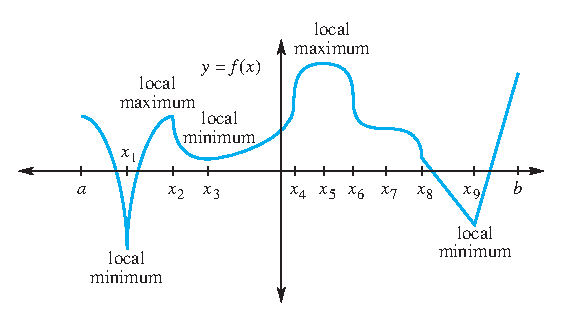
\includegraphics[width=200pt]{figsamp}
\caption[Plustech developed the first application-driven walking robot. It is designed to move
wood out of the forest. The leg coordination is automated, but navigation is still done
by the human operator on the robot.
{\tt http://www.plustech.fi/}]
{Plustech developed the first application-driven walking robot. It is designed to move
wood out of the forest. The leg coordination is automated, but navigation is still done
by the human operator on the robot.\\
{\tt http://www.plustech.fi/}}
\end{figure}

\begin{table}[!ht]
\caption{Time of the Transition Between Phase 1 and Phase 2$^{a}$}
\label{tab:label}
\begin{tabular}{lc}
\hline
 Run  & Time (min)  \\
\hline
  $l1$  & 260   \\
  $l2$  & 300   \\
  $l3$  & 340   \\
  $h1$  & 270   \\
  $h2$  & 250   \\
  $h3$  & 380   \\
  $r1$  & 370   \\
  $r2$  & 390   \\
\hline
\multicolumn{2}{l}{$^{a}$Table note text here.}
\end{tabular}
\end{table}


\subsubsection{Other Commercial Robots} 
Hostile environments such as Mars trigger
even more unusual locomotion mechanisms (figure 1.2). In dangerous and
inhospitable environments, even on Earth, such teleoperated systems have gained
popularity (figure 1.3, 1.4., 1.5). In these cases, the low-level complexities of
the robot often make it impossiblefor a human operator to directly control
its motions. The human performs localization and cognition activities, but
relays on the robot's control scheme to provide motion control stabilize the
robot submarine in spite of underwater turbulence and water currents while the
operator chooses position goals for the submarine to achieve operate not where
humans cannot go but rather share space with humans in human environments
(figure 1.6).



\section{Sample table breaking over pages}

\begin{longtable}{@{}ccc@{}}
\caption{ApJ costs from 1991 to 2013
\label{tab:table}} \\[2pt]
\hline
\bf Year & \bf Subscription & \bf Publication \\
 & \bf cost &\bf charges\\
 & \bf(\$) & \bf (\$/page)\\
\hline
\endfirsthead
\multicolumn3{@{}l}{\longtablecontinued}\\[7pt]
\hline
\bf Year & \bf Subscription & \bf Publication \\
 & \bf cost &\bf charges\\
 & \bf(\$) & \bf (\$/page)\\
\hline
\endhead
\\[12pt]
\endfoot
\hline
\\[24pt]
\endlastfoot

1991 & 600 & 100 \\
1992 & 650 & 105 \\
1993 & 550 & 103 \\
1994 & 450 & 110 \\
1995 & 410 & 112 \\
1996 & 400 & 114 \\
1997 & 525 & 115 \\
1998 & 590 & 116 \\
1999 & 575 & 115 \\
2000 & 450 & 103 \\
2001 & 490 &  90 \\
2002 & 500 &  88 \\
2003 & 450 &  90 \\
2004 & 460 &  88 \\
2005 & 440 &  79 \\
2006 & 350 &  77 \\
2007 & 325 &  70 \\
2008 & 320 &  65 \\
2009 & 190 &  68 \\
2010 & 280 &  70 \\
2011 & 275 &  68 \\
2012 & 150 &  56 \\
2013 & 140 &  55 \\
2014 & 240 &  55 \\
2015 & 245 &  50 \\
\end{longtable}


These robots are compelling not for reasons of mobility but because of their autonomy,
and so their ability to maintain a sense of position and to navigate without human intervention
is paramount For example, AGV (autonomous guided vehicle) robots (figure
1.7) autonomously deliver parts between various assembly stations by following special
electrical guidewires using a custom sensor.
\begin{equation}
N = (2k - 1) 
\end{equation}
For a biped walker k = 2 legs, the number of possible events N is using a custom
sensor. The Helpmate service robot transports food and medication
throughout hospitals
by tracking positions of ceiling lights, which are specified
\[N = 2l - 1)! = 3! = 3 � 1 = 6\]
The six different events are
\begin{enumerate}
\item
lift right leg
\item
left let leg
\item
release right leg
\item
release left leg
\item
lift both legs together
\item
release both legs together
\end{enumerate}
Of course, this quickly grows quite large. For example, a robot with six legs
has far more gaits theoretically.


\subsubsection{One Leg} The minimum number of legs a legged robot can have is, of
course, one. Minimizing the number of legs is beneficial for several reasons.
Body mass is particularly important to walking machines, and the single leg
minimizes cumulative leg mass.

Omnidirectional locomotion with three spherical wheels The omnidirectional
robot depicted in figure 2.23 is based on three spherical wheels, each actuated
by one motor. In theis design, the sperical wheels are suspended by three contact
points, two given by spherical bearings and one by a wheel connected to
the motor axle. This concept provides excellent maneuverability and is simple
in design. However, it is limited to flat surfaces and small loads, and it is quite
difficult to find round wheels with high friction coefficients.

\section{Natbib citation mark up}
Citations in the New Math book style are made using the Natbib
commands. \paragraph{Single citations}
may be made using the \verb+\citet+ or \verb+\citep+ command argument.
\vskip\baselineskip
\noindent\begin{tabular}{@{}ll}
\bf Type&\bf Results\\
\hline
\verb+\citet{jon90}+&Jones et al. (1990)\\
\verb+\citet[chap. 2]{jon90}+&Jones et al. (1990, chap. 2)\\
    \verb+\citep{jon90}+	    &   	(Jones et al., 1990)\\
    \verb+\citep[chap. 2]{jon90}+ 	&    	(Jones et al., 1990, chap. 2)\\
    \verb+\citep[see][]{jon90}+ 	 &    	(see Jones et al., 1990)\\
    \verb+\citep[see][chap. 2]{jon90}+ 	&    	(see Jones et al., 1990, chap. 2)\\
    \verb+\citet*{jon90}+ 	    &    	Jones, Baker, and Williams (1990)\\
    \verb+\citep*{jon90}+	    &    	(Jones, Baker, and Williams,
    1990) \\
\end{tabular}
\vskip\baselineskip

\paragraph{Multiple citations}
may be made by including more than one citation
key in the \verb+\citet+ or \verb+\citep+ command argument.
\vskip\baselineskip
\noindent\begin{tabular}{@{}ll}
\bf Type&\bf Results\\
\hline
\verb+\citet{jon90,jam91}+&Jones et al. (1990); James et al. (1991)\\
\verb+\citep{jon90,jam91}+&(Jones et al., 1990; James et al. 1991)\\
\verb+\citep{jon90,jon91}+&(Jones et al., 1990, 1991)\\
\verb+\citep{jon90a,jon90b}+&(Jones et al., 1990a,b)\\
\end{tabular}
\vskip\baselineskip
See \url{http://merkel.zoneo.net/Latex/natbib.php}
for a reference sheet of natbib commands.

\begin{table}[h!]
\caption{This is a table that continues over two pages.}
\begin{tabular}{lc}
\hline
 Run  & Time (min)  \\
\hline
  $l1$  & 260   \\
  $l2$  & 300   \\
  $l3$  & 340   \\
\hline
\end{tabular}
\end{table}
\clearpage
\begin{table}[h!]
\continuedcaption
\begin{tabular}{lc}
\hline
 Run  & Time (min)  \\
\hline
  $h1$  & 270   \\
  $h2$  & 250   \\
  $h3$  & 380   \\
  $r1$  & 370   \\
  $r2$  & 390   \\
\hline
\end{tabular}
\end{table}

\chapter{Gravitational Waves}
\begin{abstract}
In Einstein's theory of general relativity, gravity is treated as a
phenomenon resulting from the curvature of spacetime. This curvature
is caused by the presence of mass. Generally, the more mass that is
contained within a given volume of space, the greater the curvature of
spacetime will be at the boundary of its volume.%[12] 
\end{abstract}

\section{Mass in Spacetime}
As objects with
mass move around in spacetime, the curvature changes to reflect the
changed locations of those objects. In certain circumstances,
accelerating objects generate changes in this curvature, which
propagate outwards at the speed of light in a wave-like manner. These
propagating phenomena are known as gravitational waves.
\note{Prof. Gabriela Gonz\'alez, from Louisiana State University,
said: ``We have discovered gravitational waves from the merger of black
holes. It's been a very long road, but this is just the beginning.

Now that we have the detectors to see these systems, now that we know
binary black holes are out there - we'll begin listening to the
Universe.''}




Gravitational waves are `ripples' in the fabric of space-time caused
by some of the most violent and energetic processes in the Universe.
Albert Einstein predicted the existence of gravitational waves in 1916
in his general theory of relativity. Einstein's mathematics showed
that massive accelerating objects (such as neutron stars or black
holes orbiting each other) would disrupt space-time in such a way that
'waves' of distorted space would radiate from the source (like the
movement of waves away from a stone thrown into a pond). Furthermore,
these ripples would travel at the speed of light through the Universe,
carrying with them information about their cataclysmic origins, as
well as invaluable clues to the nature of gravity itself.
\begin{notation}
$g_{\mu\nu}(x^\lambda)=g_{\nu\mu}(x^\lambda)$&symmetric tensor\\
$g_{\mu\nu}\equiv\eta_{\mu\nu}=\mathrm{diag}(−1,1,1,1)$&Minkowski
spacetime\\
\end{notation}
The strongest gravitational waves are produced by catastrophic events
such as colliding black holes, the collapse of stellar cores
(supernovae), coalescing neutron stars or white dwarf stars, the
slightly wobbly rotation of neutron stars that are not perfect
spheres, and the remnants of gravitational radiation created by the
birth of the Universe itself.
\note{``Gravitational waves go through everything. They are hardly affected
by what they pass through, and that means that they are perfect
messengers,'' said Prof Bernard Schutz, from Cardiff University, UK.

``The information carried on the gravitational wave is exactly the same
as when the system sent it out; and that is unusual in astronomy. We
can't see light from whole regions of our own galaxy because of the
dust that is in the way, and we can't see the early part of the Big
Bang because the Universe was opaque to light earlier than a certain
time.

With gravitational waves, we do expect eventually to see the Big Bang
itself," he told the BBC.

In addition, the study of gravitational waves may ultimately help
scientists in their quest to solve some of the biggest problems in
physics, such as the unification of forces, linking quantum theory
with gravity.}


\begin{extract}
The
distance $ds$
between two neighboring events, one with coordinates
$x^\mu$
and the other
with coordinates
$x^\mu + \mathrm
{dx}^\mu+
\mathrm{dx}^\mu$, can be expressed as a function of the coordinates via a
symmetric tensor $g_{\mu\nu}(x^\lambda)=g_{\nu\mu}(x^\lambda)$
, i.e.,
\begin{equation}
\mathrm{ds}^2
=
g_{\mu\nu}
\mathrm{dx}^μ
\mathrm{dx}^\nu
\end{equation}
This is a generalization of the standard measure of distance between two points in
Euclidian space. For the Minkowski spacetime (the spacetime of special relativity),
$g_{\mu\nu}\equiv\eta_{\mu\nu}=\mathrm{diag}(−1,1,1,1)$.
(Kostas D. Kokkotas, Article for the Encyclopedia of Physical Science
and Technology, 3rd Edition, Volume 7, Academic Press, (2002)
\url{http://www.tat.physik.uni-tuebingen.de/~kokkotas/Teaching/NS.BH.GW_files/GW_Physics.pdf})
\end{extract}


Though gravitational waves were predicted to exist in 1916, actual
proof of their existence wouldn't arrive until 1974, 20 years after
Einstein's death.
Since then, many astronomers have studied the timing of pulsar radio
emissions and found similar effects, further confirming the existence
of gravitational waves. But these confirmations had always come
indirectly or mathematically and not through actual `physical'
contact.

That was the case up until September 14, 2015, when LIGO, for the
first time, physically sensed distortions in spacetime itself caused
by passing gravitational waves generated by two colliding black holes
nearly 1.3 billion light years away! LIGO and its discovery will go
down in history as one of the greatest human scientific achievements.

\section*{A Dialogue}

From the NY Times article of February 11, 2016,
{\it Gravitational Waves Detected, Confirming Einstein's Theory}\/:
\begin{dialogue}
\speaker{France C\'ordova}
It’s been decades, through a lot of different technological
innovations,
[and the foundation’s advisory board had] really scratched their heads on this one.

\speaker{Janna Levin}I was freaking out!

\speaker{Robert Garisto} [the editor of Physical Review Letters] 
I got goose bumps while reading the LIGO paper.
\end{dialogue}
The discovery is a great triumph for three physicists — Kip Thorne of
the California Institute of Technology, Rainer Weiss of the
Massachusetts Institute of Technology and Ronald Drever, formerly of
Caltech and now retired in Scotland---who bet their careers on the
dream of measuring the most ineffable of Einstein’s notions.

\begin{extract}
Gravitational waves are not sound waves, and the
general public easily could have been led to that conclusion. Sound
waves travel only through a medium such as air; ripples in spacetime
don’t need any medium to support them. Sound waves propagate at the
speed of sound; gravitational waves move at the speed of light. Even
someone with superhuman hearing could never listen in on a black hole
collision.

So why the connection between sound and gravitational waves? 
\begin{itemize}
\item LIGO detects gravitational waves with frequencies
between several hertz and several kilohertz, the sweet spot for human
hearing. 
\item When two stellar-mass black holes collide, they happen to
jiggle spacetime at the same frequency as that of pressure waves in
the air that our ears pick up as sound.     
\end{itemize}
The LIGO discovery proves that black hole binaries exist, and that
those binaries can merge within the age of the universe.
(Physics Today, April 2016 --
\url{scitation.aip.org/content/aip/magazine/physicstoday/news%
/10.1063/PT.5.2034})
\end{extract}

While the origins of gravitational waves
can be extremely violent, by the time the waves reach the Earth they
are millions of times smaller and less disruptive. In fact, by the
time gravitational waves from the first detection reached LIGO, the
amount of space-time wobbling they generated was thousands of times
smaller than the nucleus of an atom! Such inconceivably small
measurements are what LIGO was designed to make.


\begin{description}
\item[Wave passes]
As a gravitational wave passes an observer, that observer will find
spacetime distorted by the effects of strain. 

\item[Distances]
Distances between
objects increase and decrease rhythmically as the wave passes, at a
frequency corresponding to that of the wave. 
\end{description}
This occurs despite such
free objects never being subjected to an unbalanced force. The
magnitude of this effect decreases proportional to the inverse
distance from the source.
\begin{outline}
\begin{enumerate}
\item[I.]
 Inspiraling binary neutron
stars are predicted to be a powerful source of gravitational waves as
they coalesce, due to the very large acceleration of their masses as
they orbit close to one another. 

\item[II.]
However, due to the astronomical
distances to these sources, the effects when measured on Earth are
predicted to be very small, having strains of less than 1 part in
1020. 

\begin{enumerate}
\item[A.]
Scientists have demonstrated the existence of these waves with
ever more sensitive detectors. 

\begin{enumerate}
\item[1.]
The most sensitive detector
accomplished the task possessing a sensitivity measurement of about
one part in 5$\times$1022 (as of 2012) provided by the LIGO and VIRGO
observatories.

\item[2.]
A space based observatory, the Laser Interferometer
Space Antenna, is currently under development by ESA. 
\end{enumerate}
\item[B.]
Gravitational waves can penetrate regions of space that
electromagnetic waves cannot. 
\end{enumerate}
\item[III.]
They are able to allow the observation
of the merger of black holes and possibly other exotic objects in the
distant Universe. 
\end{enumerate}
\end{outline}
Such systems cannot be observed with more
traditional means such as optical telescopes or radio telescopes, and
so gravitational-wave astronomy gives new insights into the working of
the Universe. In particular, gravitational waves could be of interest
to cosmologists as they offer a possible way of observing the very
early Universe. This is not possible with conventional astronomy,
since before recombination the Universe was opaque to electromagnetic
radiation.

Precise measurements of gravitational waves will also
allow scientists to more thoroughly test the general theory of
relativity.

\begin{boxedtext}{Frank Wilczek on Einstein and Gravitation}
Einstein's general relativity, as a theory of gravitation, is so tight
conceptually that it allows only two free parameters: Newton’s
constant and the cosmological term. It has passed every test that
physicists and astronomers have devised. Yet there are reasons to
remain dissatisfied.

\section{First}
First, the strength of gravity is grossly disproportionate to the
strength of other forces. If we believe in the unity of nature’s
operating system, how can that be? 

\subsection{Second}
Second, the measured value of the
mass density of space devoid of matter---the cosmological term, often
called dark energy---is incommensurate with reasonable expectations. Why
is it much smaller than theory suggests, yet not zero? 

\subsubsection{Third}
Third, the
equations that follow from straightforward quantization of general
relativity break down in extreme conditions. What are the
consequences? Those issues are important agenda items for the next 100
years of physics. In the boxes, I've indicated a promising way to
approach the question of the weakness of gravity. Here I'll offer a
few comments on the other issues.

\begin{extract}
Theorists have estimated several contributions to the cosmological
term-positive and negative---whose individual absolute values far exceed
the observed total value. Thus the term’s observed smallness indicates
delicate cancellations that our core theories do not explain. Perhaps,
as suggested by Steven Weinberg, the explanation is anthropic. Too
large a cosmological term would lead the universe to expand so rapidly
that formation of structure in the universe would be inhibited.
Neither galaxies nor stars nor planets would form, and thus observers
could not emerge. Is that anthropic argument the best physics can
do---is resistance futile? Or is some deeper principle at work?
\end{extract}

\section*{Conceptual difficulty}
The conceptual difficulty of reconciling our theory of gravity,
general relativity, with the principles of quantum mechanics has been
the subject of much hyperbole. I think it is important, therefore,
first to bring it down to earth.   

(Frank Wilczek, Physics Today, April 2016,
\url{scitation.aip.org/content/aip/magazine/physicstoday/article/69/4/10.1063/PT.3.3137})
\end{boxedtext}

In principle, gravitational waves could exist at any frequency.
However, very low frequency waves would be impossible to detect and
there is no credible source for detectable waves of very high
frequency. Stephen Hawking and Werner Israel list different frequency
bands for gravitational waves that could plausibly be detected,
ranging from 10--7 Hz up to 1011 Hz. 
\blankline
\begin{tabular}{l|l}    
\hline
\multicolumn2c{\bf Acceleration Equations}\\
\hline
\it With initial velocity&\it Starting from rest\\
\hline
$v_f=v_i+ a \Delta\, t$&$v_f=a\Delta\, t$\\
$\Delta\, d=v_i \Delta\, t + 1/2 a \Delta\, t^2$&
$\Delta\, d= 1/2 a \Delta\, t^2$\\
$v_f=\sqrt{v_i^2+2a\Delta\, d}$&
$v_f=\sqrt{2a\Delta\, d}$\\[6pt]
\hline
\end{tabular}
\blankline
In theory, the loss of energy through gravitational radiation could
eventually drop the Earth into the Sun. However, the total energy of
the Earth orbiting the Sun (kinetic energy + gravitational potential
energy) is about 1.14$\times$1036 joules of which only 200 joules per second
is lost through gravitational radiation, leading to a decay in the
orbit by about $1\times10$--15 meters per day or roughly the diameter of a
proton. At this rate, it would take the Earth approximately $1\times 1013$
times more than the current age of the Universe to spiral onto the
Sun. This estimate overlooks the decrease in r over time, but the
majority of the time the bodies are far apart and only radiating
slowly, so the difference is unimportant in this example.
\vskip\baselineskip
\noindent
\begin{tabular*}{\textwidth}{@{\extracolsep\fill}cc@{}}    
\hline
\multicolumn2c{\bf Acceleration Equations}\\
\hline
\it With initial velocity&\it Starting from rest\\
\hline
$v_f=v_i+ a \Delta\, t$&$v_f=a\Delta\, t$\\
$\Delta\, d=v_i \Delta\, t + 1/2 a \Delta\, t^2$&
$\Delta\, d= 1/2 a \Delta\, t^2$\\
$v_f=\sqrt{v_i^2+2a\Delta\, d}$&
$v_f=\sqrt{2a\Delta\, d}$\\[6pt]
\hline
\end{tabular*}
\vskip\baselineskip

\begin{table}
\caption{A table of acceleration equations.}
\begin{tabular}{l|l}    
\hline
\it With initial velocity&\it Starting from rest\\
\hline
$v_f=v_i+ a \Delta\, t$&$v_f=a\Delta\, t$\\
$\Delta\, d=v_i \Delta\, t + 1/2 a \Delta\, t^2$&
$\Delta\, d= 1/2 a \Delta\, t^2$\\
$v_f=\sqrt{v_i^2+2a\Delta\, d}$&
$v_f=\sqrt{2a\Delta\, d}$\\[6pt]
\hline
\end{tabular}
\end{table}

More generally, the rate of orbital decay can be approximated by [32].
\[
    \frac{\mathrm{d}r}{\mathrm{d}t} = - \frac{64}{5}\,
    \frac{G^3}{c^5}\, \frac{(m_1m_2)(m_1+m_2)}{r^3}\ ,  
\]
where $r$ is the separation between the bodies, $t$ time, G Newton's
constant, $c$ the speed of light, and $m1$ and $m2$ the masses of the
bodies. This leads to an expected time to merger of 
\begin{equation}
    t= \frac{5}{256}\, \frac{c^5}{G^3}\,
    \frac{r^4}{(m_1m_2)(m_1+m_2)}.  
\end{equation}
For example a pair of solar mass neutron stars in a circular orbit at
a separation of $1.89\times108$ $m$ (189,000 km) has an orbital
period of 1,000 


\begin{boxedtext}{Two Theorems and a Corollary}
 	
\begin{theorem}[Birkhoff's Theorem]
The metric of the Schwarzschild black hole is the unique spherically
symmetric solution of the vacuum {\it Einstein field equations}.
\[G^{\mu\nu}=0.\]

Stated another way, a spherically symmetric gravitational field in
empty space must be static, with a metric given by the Schwarzschild
black hole metric.
\end{theorem}

\begin{corollary}
A corollary states that the metric inside a spherical cavity inside a
spherical mass distribution is the Minkowski metric. 
\end{corollary}

\begin{theorem}[Schwarzschild Black Hole]
 A black hole with zero charge $Q = 0$ and no angular momentum $J = 0$.
The exterior solution for such a black hole is known as the
Schwarzschild solution (or Schwarzschild metric), and is an exact
unique solution to the Einstein field equations of general relativity
for the general static isotropic metric (i.e., the most general metric
tensor that can represent a static isotropic gravitational field), 
\[
d\tau^2=B(r)dt^2 - A(r)dr^2-r^2 \sin^2\theta\, d\phi^2.
\]
\end{theorem}
In 1915, when Einstein first proposed them, the 
Einstein field equations appeared so complicated that he did not 
believe that a solution would ever be found. 
He was therefore quite surprised when, only a year later, 
Karl Schwarzschild  (1916) discovered one by making the assumption of
spherical symmetry. 
\end{boxedtext}



\section{Samples of Programming Code}

\begin{code}
\begin{verbatim}
procedure bubbleSort( A : list of sortable items )
    n = length(A)
    repeat
       newn = 0
       for i = 1 to n-1 inclusive do
          if A[i-1] > A[i] then
             swap(A[i-1], A[i])
             newn = i
          end if
       end for
       n = newn
    until n = 0
end procedure
\end{verbatim}
\end{code}

\newpage
\noindent
Algorithm environment:


%% \begin{algorithm} takes option [p][b][t][h],  or some combination, like \begin{figure}
\begin{algorithm}[h]
\caption{A sample in an algorithm environment.}
\begin{algorithmic}
\If {$i\geq maxval$}
    \State $i\gets 0$
\Else
    \If {$i+k\leq maxval$}
        \State $i\gets i+k$
    \EndIf
\EndIf
\end{algorithmic}
\end{algorithm}

\begin{boxedtext}{Two examples  of Programming Code}
\begin{code}
\begin{verbatim}
procedure bubbleSort( A : list of sortable items )
    n = length(A)
    repeat
       newn = 0
       for i = 1 to n-1 inclusive do
          if A[i-1] > A[i] then
             swap(A[i-1], A[i])
             newn = i
          end if
       end for
       n = newn
    until n = 0
end procedure
\end{verbatim}
\end{code}
And
\begin{algorithmic}
\If {$i\geq maxval$}
    \State $i\gets 0$
\Else
    \If {$i+k\leq maxval$}
        \State $i\gets i+k$
    \EndIf
\EndIf
\end{algorithmic}
\end{boxedtext}

\newpage
\begin{exercises}
\exer{For Hooker's data, Exercise 1.2, use the Box and Cox and Atkinson procedures to determine a appropriate transformation of PRES
in the regression of PRES on TEMP. find $\hat\lambda$, $\tilde\lambda$,
the score test, and the added variable plot for the score. 
Summarize the results.}

\subexer{The following data were collected in a study of the effect of dissolved sulfur
on the surface tension of liquid copper (Baes and Killogg, 1953).}


\blankline
\begin{tabular}{r@{}lcc}
\hline
&&\multicolumn2c{$Y$= Decrease in Surface Tension}\\
\multicolumn2c{$x$ = Weight \% sulfur}
&\multicolumn2c{(dynes/cm), two Replicates}\\
\hline
0.&034&301&316\\
0.&093&430&422\\
011.&30&593&586\\
\hline
\end{tabular}
\blankline

\subexer{Find the transformations of $X$ and $Y$ sot that in the transformed scale 
the regression is linear.}

\subexer{Assuming that $X$ is transformed to $\ln(X)$, which choice of $Y$ gives 
better results,
$Y$ or $\ln(Y)$? (Sclove, 1972).}

\sidebysidesubsubexer{In the case of $\Delta_1$?}{In the case of $\Delta_2$?}

\exer{Examine the Longley data, Problem 3.3, for applicability of assumptions of the
linear model.}

\sidebysidesubexer{In the case of $\Gamma_1$?}{In the case of $\Gamma_2$?}
\[
    t= \frac{5}{256}\, \frac{c^5}{G^3}\,
    \frac{r^4}{(m_1m_2)(m_1+m_2)}.  
\]

\end{exercises}



\begin{chapappendix}{Dark Matter is not composed of Black Holes}

\section{The Canada France Hawaii Lensing Survey}

Did you know that less than 4\% of our Universe is made up of regular
matter - the type that makes up the Earth, the planets and the stars?
The rest is 'dark' and invisible, but we know that it is there through
its effects on the regular matter that we can see. The gravity of Dark
Matter causes galaxies to clump together in a giant cosmic web, and
Dark Energy is pushing space itself apart at an accelerated rate. With
some of the world's best telescopes we can directly witness the
ongoing battle between these two strange entities.

\subsection{CFHTL}
The Canada-France-Hawaii Telescope Lensing Survey uses an innovative
technique called gravitational lensing to observe the invisible dark
matter in our Universe. Using data accumulated over five years by the
CFHT Legacy Survey, the CFHTLenS team have analysed the images of over
10 million galaxies. The light emitted by these galaxies has taken
nearly half the age of the Universe to reach us and has been bent and
distorted by the massive clumps of dark matter it has passed by.
Exploiting this fact that `mass bends light', as predicted by
Einstein, we have privileged access to the mysterious components of
the Universe that cannot otherwise be observed.

%Author: Emma Grocutt

\section{Dark Matter and Black Holes}
We know that dark matter exists because of our mathematical graphs of
how fast the material in a galaxy is rotating in relation to the
center of the galaxy (where most of the galactic material is located).
And as a result of these graphs, we know that dark matter surrounds
galaxies. In the end, the farther out you go, the more mass
grows\ldots and
it grows by a lot. So in short, we know that dark matter isn’t just
some black hole that exists out in the middle of intergalactic space
based on the way that galaxies rotate and evolve over time.

 As Emma Grocutt, from the
CFHTL Survey notes:

\begin{extract}
``The most interesting thing about dark matter is not simply that we
can't see it, it's that we know dark matter is not made of the same
stuff as normal baryonic matter. This is actually why we can't see
it---baryons interact with each other through gravity, nuclear forces and
the electrostatic force. These interactions are what allow baryonic
matter (such as stars) to emit light, and what prevent you from
putting your hand through a table---the particles of your hand are
electrostatically repelled from the particles in the table. Dark
matter, however, only interacts through gravity. This is why we see
its effects on the motions of galaxies and stars, but why we can't see
it directly; it does not emit or absorb light. Dark matter particles
can also pass through regular matter almost completely undetected
since they don't interact electrostatically, meaning we can't touch it
or sense it in any direct way.''
(\url{http://futurism.com/the-quest-for-dark-matter-could-the-missing-universe-be-black-holes-2/})
\end{extract}

\end{chapappendix}


\chapternotes


\appendix
\chapter{Evaluating the significance of the proof of gravity
waves} 

\section{On a par with determination of structure of DNA}
Prof Karsten Danzmann, from the Max Planck Institute for
Gravitational Physics and Leibniz University in Hannover, Germany, is
a European leader on the collaboration.\footnote{Text and graphics
from
\url{http://www.bbc.com/news/science-environment-35524440}}


He said the detection was one of the most important developments in
science since the discovery of the Higgs particle, and on a par with
the determination of the structure of DNA.


``There is a Nobel Prize in it---there is no doubt,'' he told the BBC.

\begin{figure}[h!]

\includegraphics[width=\textwidth]{gravwaves}
\caption{Graphic showing two black holes generating gravity waves.}
\end{figure}




``It is the first ever direct detection of gravitational waves; it's
the first ever direct detection of black holes and it is a
confirmation of General Relativity because the property of these black
holes agrees exactly with what Einstein predicted almost exactly 100
years ago.''
\begin{equation}
d\tau^2=B(r)dt^2 - A(r)dr^2-r^2 \sin^2\theta\, d\phi^2.
\end{equation}

\begin{figure}[p]
\rotatebox{90}{\hskip-3in\vbox {
\includegraphics[width=\textheight]{gravwaves}
\caption{(landscape figure)
Graphic showing two black holes generating gravity waves.}}}
\end{figure}
\clearpage

\begin{table}[p]
\rotatebox{90}{\vbox{
\caption{More relevant tabular information.\label{tbl-2}}
\begin{tabular}{@{}crrrrrrrrrrr}
\hline
Star & Height & $d_{x}$ & $d_{y}$ & $n$ & $\chi^2$ & $R_{maj}$ & $R_{min}$ &
\multicolumn{1}{c}{$P^a$} & $P R_{maj}$ & $P R_{min}$ &
\multicolumn{1}{c}{$\Theta^b$} \\
\hline
1 &33472.5 &-0.1 &0.4  &53 &27.4 &2.065  &1.940 &3.900 &68.3 &116.2 &-27.639\\
2 &27802.4 &-0.3 &-0.2 &60 &3.7  &1.628  &1.510 &2.156 &6.8  &7.5 &-26.764\\
3 &29210.6 &0.9  &0.3  &60 &3.4  &1.622  &1.551 &2.159 &6.7  &7.3 &-40.272\\
4 &32733.8 &-1.2\rlap{$^c$} &-0.5 &41 &54.8 &2.282  &2.156 &4.313 &117.4 &78.2 &-35.847\\
5 & 9607.4 &-0.4 &-0.4 &60 &1.4  &1.669\rlap{$^c$} &1.574 &2.343 &8.0  &8.9 &-33.417\\
6 &31638.6 &1.6  &0.1  &39 &315.2 & 3.433 &3.075 &7.488 &92.1 &25.3 &-12.052\\
\hline\\
\multicolumn{12}{l}{$^a$
Sample footnote for table~\ref{tbl-2} that was
generated with the \LaTeX\ table environment}\\
\multicolumn{12}{l}{$^b$ Yet another sample footnote for table
\ref{tbl-2}}\\
\multicolumn{12}{l}{$^c$ Another sample footnote for
table~\ref{tbl-2}}\\
\end{tabular}}}
\end{table}


\section{Ripples in the fabric of space-time}

\begin{itemize}
\item
    Gravitational waves are a prediction of the Theory of General
    Relativity 
\item
    Their existence has been inferred by science but only now
    directly detected 
\item
    They are ripples in the fabric of space and time produced by
    violent events 
\item
    Accelerating masses will produce waves that propagate at the
    speed of light 
\item
    Detectable sources ought to include merging black holes and
    neutron stars 
\item
    Ligo fires lasers into long, L-shaped tunnels; the waves disturb
    the light 
\item
    Detecting the waves opens up the Universe to completely new
    investigations 
\end{itemize}


\subsection{Stephen Hawking Agrees on Importance}
That view was reinforced by Prof Stephen Hawking, who is an expert on
black holes.\footnote{Perhaps somewhat immodestly, 
this claim is made
on Hawking's website (\url{www.hawking.org.uk}):
``Stephen Hawking is regarded as one of the
most brilliant theoretical  physicists since Einstein.''
Though, of course, it may well be true!}
Speaking exclusively to BBC News, he said he believed
that the detection marked a key moment in scientific history.
\note{Stephen Hawking said that the detection of gravity waves
marked a key moment in scientific history.}


``Gravitational waves provide a completely new way at looking at the
Universe. The ability to detect them has the potential to
revolutionise astronomy. This discovery is the first detection of a
black hole binary system and the first observation of black holes
merging,'' he said.

``Apart from testing (Albert Einstein's theory of) General Relativity,
we could hope to see black holes through the history of the Universe.
We may even see relics of the very early Universe during the Big Bang
at some of the most extreme energies possible.''

\subsection{Too beautiful to be true?}
We found a beautiful signature of the merger of two black holes and
it agrees exactly - fantastically - with the numerical solutions to
Einstein equations... it looked too beautiful to be true," said Prof
Danzmann.\index{beauty}\index{truth}\index{truth and
beauty!truth}\index{beauty and truth!beauty}

\endmatter

\begin{glossary}
\term{Absolute Zero}{
The lowest temperature possible, equivalent to -273.15$^{\deg}$C (or
0$^{\deg}$ on the
absolute Kelvin scale), at which point atoms cease to move altogether
and molecular energy is minimal. The idea that it is impossible,
through any physical process, to lower the temperature of a system to
zero is known as the Third Law of Thermodynamics.}


\term{Alpha Particle (Alpha Decay)}{
A particle of 2 protons and 2 neutrons (essentially a helium nucleus)
that is emitted by an unstable radioactive nucleus during radioactive
decay. It is a relatively low-penetration particle due its
comparatively low energy and high mass.}

\term{Angular Momentum}{A measure of the momentum of a body in rotational
motion about its centre of mass. Technically, the angular momentum of
a body is equal to the mass of the body multiplied by the cross
product of the position vector of the particle with its velocity
vector. The angular momentum of a system is the sum of the angular
momenta of its constituent particles, and this total is conserved
unless acted on by an outside force.}

\term{Anthropic Principle}
{The idea that the fundamental constants of physics and chemistry are
just right (or ``fine-tuned'') to allow the universe and life as we know
it to exist, and indeed that the universe is only as it is because we
are here to observe it. Thus, we find ourselves in the kind of
universe, and on the kind of planet, where conditions are ripe for our
form of life.}

\term{Antimatter}{Pair production and pair annihilation
of hydrogen and antihydrogen particles. 
A large
accumulation of antiparticles---antiprotons, antineutrons and
positrons (antielectrons)---which have opposite properties to normal
particles (e.g. electrical charge), and which can come together to
make antiatoms. When matter and antimatter meet, they self-destruct in
a burst of high-energy photons or gamma rays. The laws of physics seem
to predict a pretty much 50/50 mix of matter and antimatter, despite
the observable universe apparently consisting almost entirely of
matter, known as the ``baryon asymmetry problem''.}

%(Source: Riken Research:
%\url{http://www.rikenresearch.riken.jp/eng/frontline/5444})\\ 

\end{glossary}

\begin{endbookexercises}
\exer{For Hooker's data, Exercise 1.2, use the Box and Cox and Atkinson procedures to determine a appropriate transformation of PRES
in the regression of PRES on TEMP. find $\hat\lambda$, $\tilde\lambda$,
the score test, and the added variable plot for the score. 
Summarize the results.}

\subexer{The following data were collected in a study of the effect of dissolved sulfur
on the surface tension of liquid copper (Baes and Killogg, 1953).}
\blankline
\begin{tabular}{rlcc}
\hline
&&\multicolumn2c{$Y$= Decrease in Surface Tension}\\
\multicolumn2c{$x$ = Weight \% sulfur}
&\multicolumn2c{(dynes/cm), two Replicates}\\
\hline
0.&034&301&316\\
0.&093&430&422\\
0.&30&593&586\\
\hline
\end{tabular}
\blankline


\subexer{Find the transformations of $X$ and $Y$ sot that in the transformed scale 
the regression is linear.}

\subexer{Assuming that $X$ is transformed to $\ln(X)$, which choice of $Y$ gives 
better results,
$Y$ or $\ln(Y)$? (Sclove, 1972).}

\sidebysidesubsubexer{In the case of $\Delta_1$?}{In the case of $\Delta_2$?}

\exer{Examine the Longley data, Problem 3.3, for applicability of assumptions of the
linear model.}

\sidebysidesubexer{In the case of $\Gamma_1$?}{In the case of $\Gamma_2$?}

\[
    t= \frac{5}{256}\, \frac{c^5}{G^3}\,
    \frac{r^4}{(m_1m_2)(m_1+m_2)}.  
\]

\end{endbookexercises}

\endnotes

%% \nocite{*} is a way to get all the entries in the .bib file to print in the bibliography:
\nocite{*}
\bibliographystyle{mit-chicago}
\bibliography{bibsamp}

\printindex

\end{document}

